\chapter{La realizzazione della struttura centrale}

Terminata l'analisi del problema, che ne ha stabilito i requisiti, le funzionalità e la struttura generale,
si passa alla fase di progettazione.
Durante questa fase l'obiettivo principale è identificare le caratteristiche funzionali e comportamentali del sistema, 
delineando le componenti principali e le rispettive responsabilità.
Questo permette di definire un'architettura coerente, 
facilitando le successive scelte tecnologiche e implementative.\\
\\
Nella fase successiva, di implementazione, 
si procede con il passaggio dall’analisi teorica alla realizzazione concreta,
dove la selezione dell’architettura e delle tecnologie di riferimento assumono un ruolo centrale.
Le decisioni prese in questa fase determinano il comportamento dei diversi componenti e 
le modalità con cui essi interagiscono tra loro.
Un’attenta selezione delle soluzioni ottimali, più adatte ai requisiti definiti in fase di progettazione,
permette di impostare fin dalle prime iterazioni uno sviluppo efficiente e strutturato, 
minimizzando la necessità di revisioni successive.\\
\\
Nonostante alcune decisioni risultino immediate o intercambiabili, 
altre richiedono analisi approfondite per individuare la soluzione più adatta.
Un approccio efficace consiste nello sviluppare inizialmente i componenti con requisiti ben definiti,
per poi affinare progressivamente l'integrazione e la configurazione con gli altri elementi del sistema.
L'identificazione, anche parziale, di una struttura iniziale consente di delineare i vincoli di integrazione e 
di semplificare la definizione delle soluzioni residue.\\
\\
L’architettura dell’applicativo si basa su una chiara suddivisione in componenti, 
ciascuno con un ruolo specifico all’interno del sistema.
\\

Tale organizzazione modulare consente di ottimizzare la scalabilità e la manutenibilità dell’applicativo,
facilitando eventuali evoluzioni future.
La suddivisione chiara delle responsabilità, unita a un’architettura flessibile e sicura,
rappresenta quindi un elemento chiave per garantire la stabilità e l’efficienza del sistema nel lungo periodo.\\
\\
\begin{figure}[htb]
    \centering
    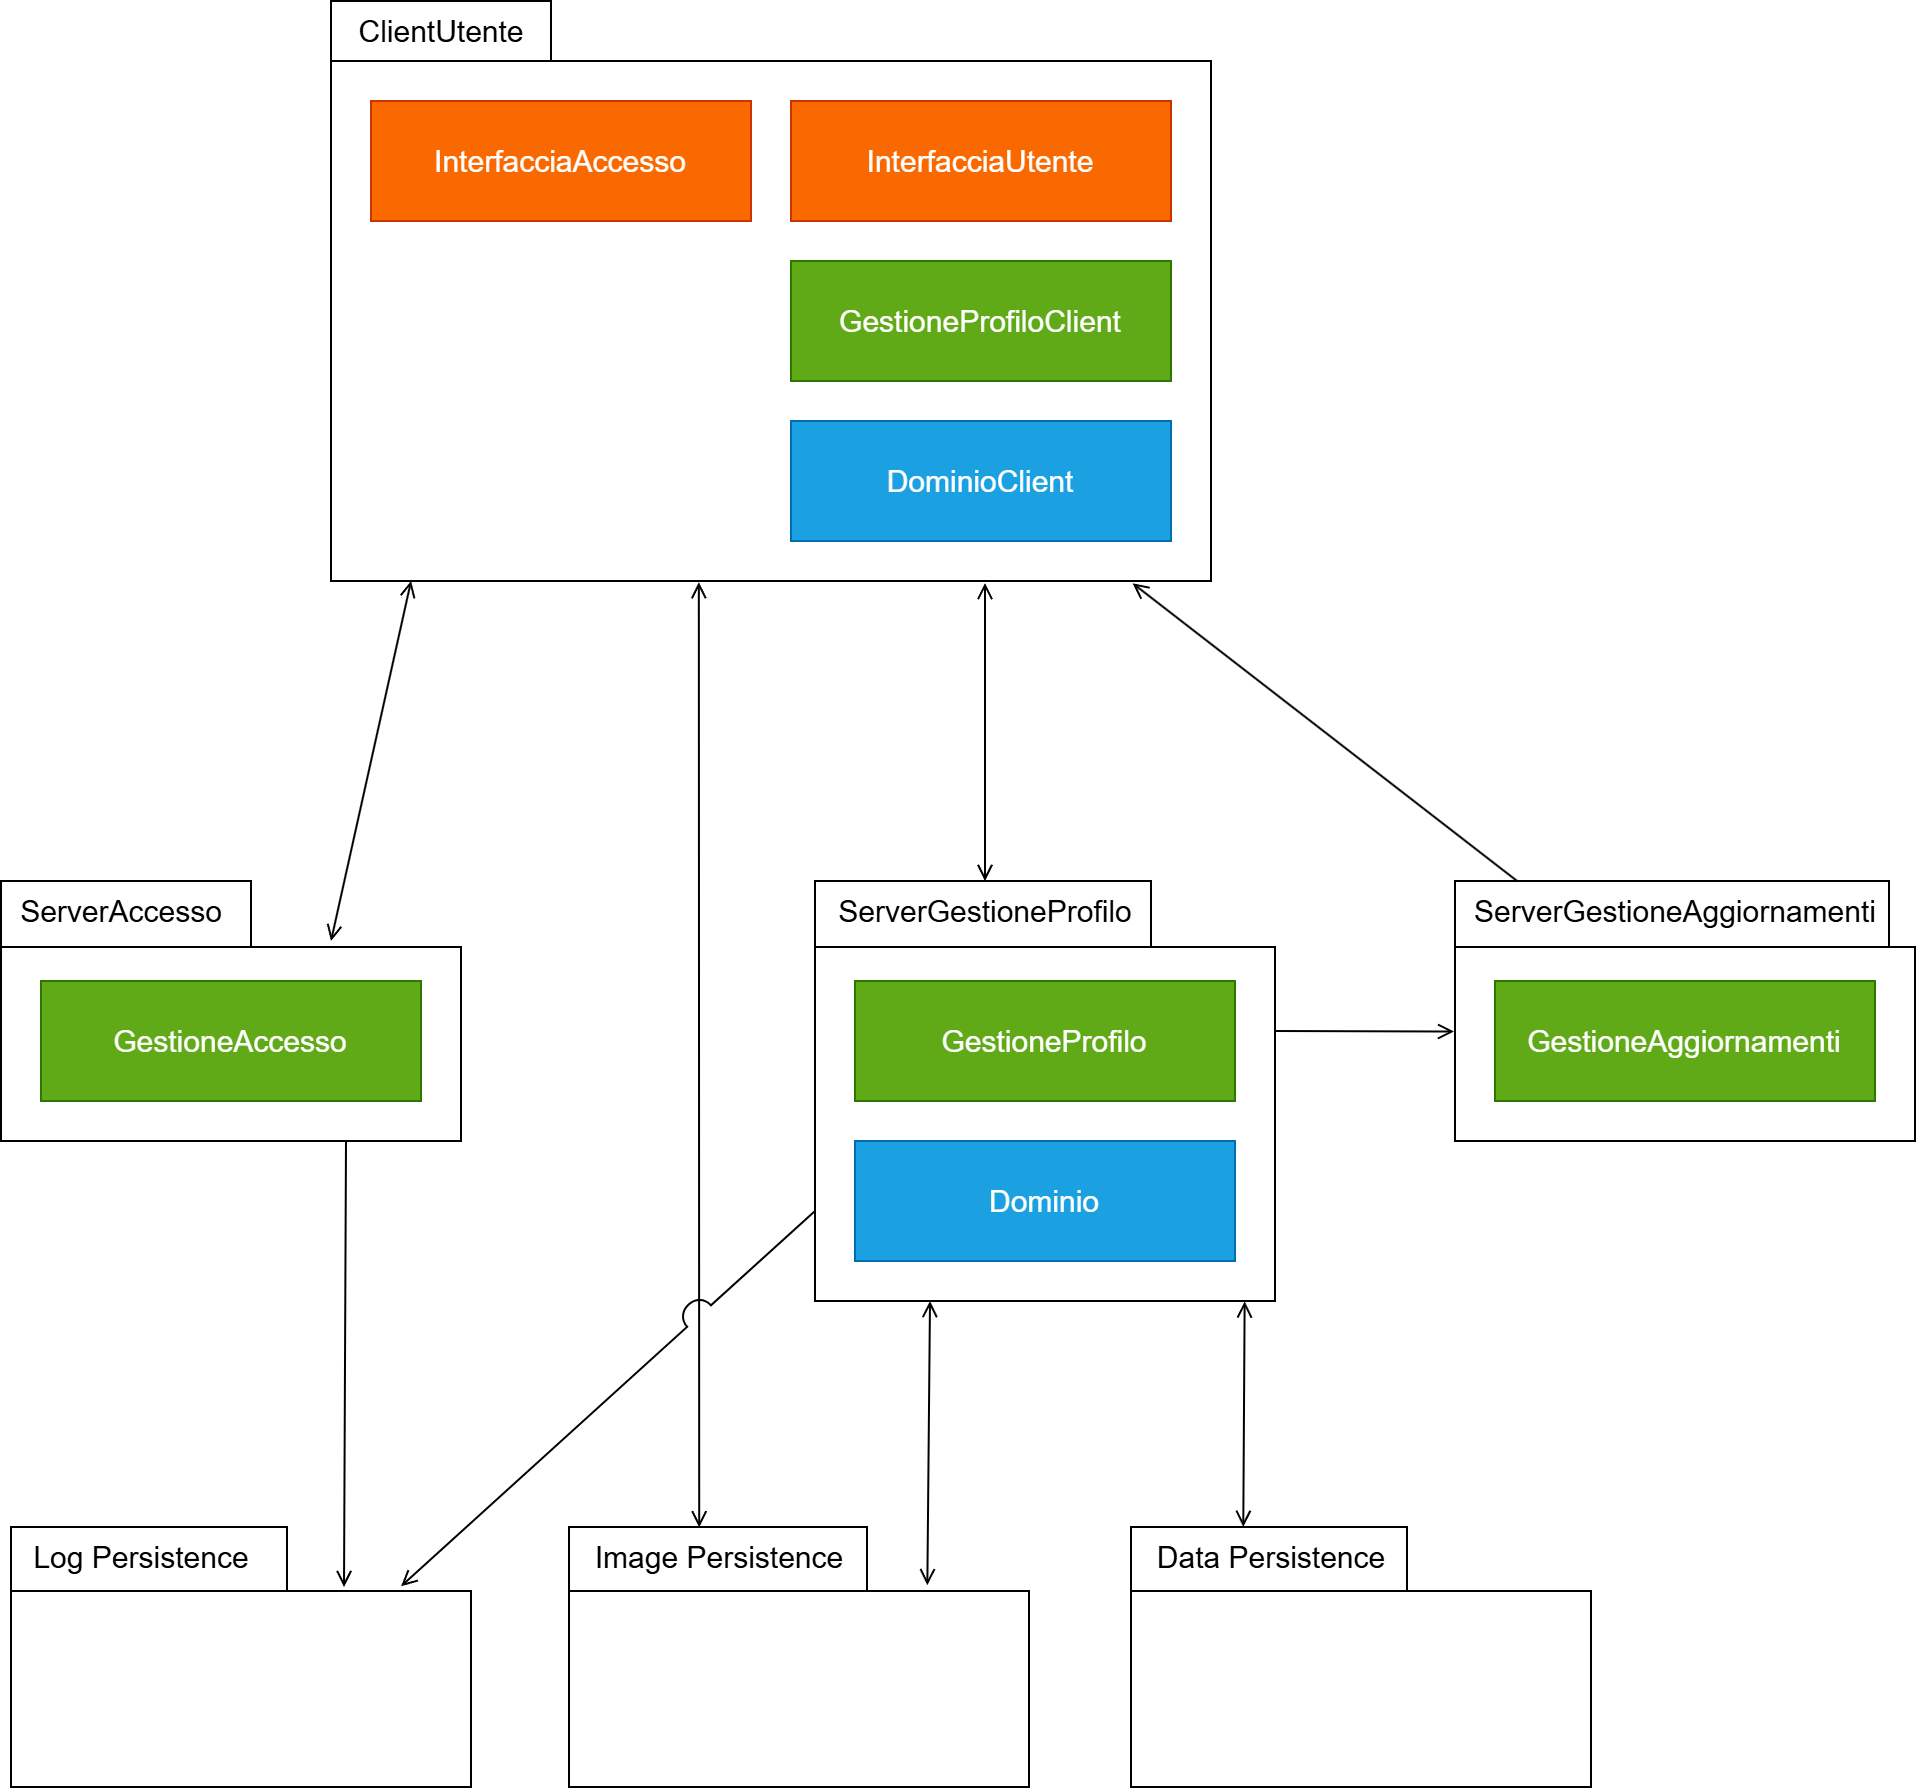
\includegraphics[height=0.67\textheight]{ProgettoDiagrammaPackage.png}
    \caption{Struttura e responsabilità delle parti del progetto}
\end{figure}
\clearpage
L'interfaccia grafica è responsabile della presentazione e dell’interazione con l’utente, 
ponendo particolare attenzione alla coerenza visiva e alla fluidità dell’esperienza.
La logica applicativa sarà gestita da un server dedicato, 
il quale si occupa di coordinare le comunicazioni tra i diversi servizi
e di garantire il corretto flusso delle operazioni.
La gestione dell’autenticazione degli utenti verrà separata dal resto del sistema, 
delegando questa responsabilità a un servizio apposito,
per migliorare sia le prestazioni che la sicurezza.\\
\\
Un ulteriore aspetto fondamentale nella progettazione del sistema riguarda 
la protezione delle comunicazioni e dei dati sensibili.
L’adozione di misure di sicurezza adeguate è essenziale per garantire la protezione delle informazioni scambiate tra i vari componenti e
per ridurre i rischi derivanti da eventuali attacchi esterni.
Inoltre, per monitorare il corretto funzionamento dell’applicazione e 
identificare tempestivamente eventuali anomalie,
il sistema è integrato con strumenti di logging e analisi delle prestazioni.\\
\\
Già consolidata e affidabile, sin dalle prime fasi di sviluppo del progetto è stata adottata la piattaforma cloud Azure, per garantire un'infrastruttura solida e scalabile.\\
\\

\section{Lo sviluppo del client utente}

L’utilizzo delle applicazioni per la gestione degli eventi può essere suddiviso in due fasi distinte, 
ciascuna con specifiche esigenze funzionali.\\
\\
La prima fase riguarda la pianificazione a lungo termine e l’organizzazione degli impegni.
In questa circostanza l’utente decide come distribuire il proprio tempo, pianificando attività e appuntamenti,
e strutturando il proprio calendario nel modo più efficiente per le proprie necessità.
La seconda fase riguarda invece la gestione degli eventi non ancora certi e definiti;
ciò include l’invito a un evento, l’eventuale conferma da parte dell’utente,
l’identificazione degli impegni a breve termine e l’aggiornamento del loro stato
(ad esempio, se l’evento sia ancora confermato, quante persone vi partecipano, se qualcuno ha annullato o se l'evento è già concluso)
con la gestione degli eventuali contenuti multimediali successivi all’evento. 
Queste due fasi implicano un approccio diverso da parte dell’utente,
comportando di conseguenza esigenze differenti a cui l’applicazione deve rispondere adeguatamente.\\
\\
Per rispondere a tali necessità, è fondamentale che l'applicazione offra un'interfaccia utente versatile, 
fruibile sia da desktop che da dispositivi mobili.
La versione desktop consente una pianificazione a lungo termine, offrendo una visione d'insieme chiara e completa di tutti gli impegni,
tale da facilitare la gestione del tempo.
D'altra parte, la versione mobile deve permettere una gestione rapida e dinamica degli eventi quotidiani,
garantendo che l'utente possa rimanere sempre connesso e aggiornato sugli sviluppi in tempo reale.\\
\\
Inoltre, considerando che l'applicazione è destinata a un utilizzo diffuso e a un'utenza potenzialmente elevata,
è necessario garantire tempi di risposta ridotti e una gestione efficiente delle richieste concorrenti.
Ciò implica la progettazione di un sistema in grado di scalare facilmente,
per supportare un ampio numero di utenti simultanei senza compromettere le prestazioni.\\
\\

\subsection{La scelta del framework di sviluppo}

Al fine di ottenere tutte le prestazioni precedentemente elencate, 
la scelta è ricaduta sull’adozione del framework di sviluppo Flutter.
Diversi fattori motivano tale decisione. \\
\\
In primo luogo, l'architettura di Flutter si basa su un motore grafico 
indipendente dalla piattaforma di esecuzione,
il che consente di ottenere elevate prestazioni e 
garantire un'esperienza utente uniforme su dispositivi diversi.
In secondo luogo, Flutter adotta un approccio dichiarativo nella progettazione dell'interfaccia grafica,
che facilita lo sviluppo di componenti reattivi attraverso un codice conciso, facilmente mantenibile.\\
\\
Un ulteriore vantaggio di Flutter è rappresentato dalla crescente adozione nel settore,
dalla solidità della community di sviluppo e dal supporto offerto da Google,
che ne assicurano la stabilità, l'efficienza, la sicurezza e la disponibilità 
di componenti personalizzabili per l'intero ciclo di vita del prodotto.
Infine, Flutter consente uno sviluppo rapido e interattivo 
grazie alla sua sintassi intuitiva e al meccanismo di hot reload,
che riduce significativamente i tempi di compilazione e facilita il testing in tempo reale.\\
\\
Tra le altre tecnologie valutate per lo sviluppo dell'interfaccia grafica vi erano React Native e Xamarin.
Tuttavia, entrambe presentano alcune limitazioni: 
le applicazioni finali sviluppate con React Native tendono ad avere dimensioni più elevate e le prestazioni risultano inferiori,
in particolare nella gestione della memoria.
Xamarin, pur essendo una valida opzione, presenta una curva di apprendimento più ripida e 
una comunità di sviluppatori ridotta rispetto a Flutter,
con una conseguente minore disponibilità di componenti e librerie.\\
\\
L'applicazione utente ha come obiettivo la soddisfazione di due compiti principali: 
interagire con l'utente e comunicare con il server, 
per recuperare i dati e salvare le modifiche apportate.\\
\\

\subsection{La realizzazione delle interfacce grafiche}
L'interazione utente avviene tramite interfacce grafiche 
che permettono di visualizzare i dati e le funzionalità a disposizione. 
Per rispettare il requisito di semplicità e fluidità dell'esperienza è essenziale che 
ogni interfaccia sia il più intuitiva possibile, tramite una limitata varietà di azioni nella stessa pagina,
ognuna delle quali facilmente accessibile, ma anche riconoscibile in base alla sua importanza e funzionalità.\\
\\
Per ogni maschera individuata in fase di analisi corrisponde almeno un'interfaccia grafica che, 
oltre a gestire la navigazione con le altre interfacce, 
permette all'utente di eseguire le proprie funzionalità,
esponendo chiaramente le informazioni,
concentrando l'attenzione sui dati eventualmente richiesti e segnalando le azioni eseguibili.\\
\\
Nei diagrammi di dettaglio le interfacce vengono presentate elencando le funzionalità di cui dispongono, 
assieme alle loro relazioni di dipendenza.
Si riportano le interfacce di gestione dei gruppi e di visualizzazione degli eventi, 
in quanto funzionalità centrali, il cui stile grafico è stato rispettato nella creazione del resto dell'applicazione.\\
\\
\begin{figure}[htbp]
    \begin{center}
        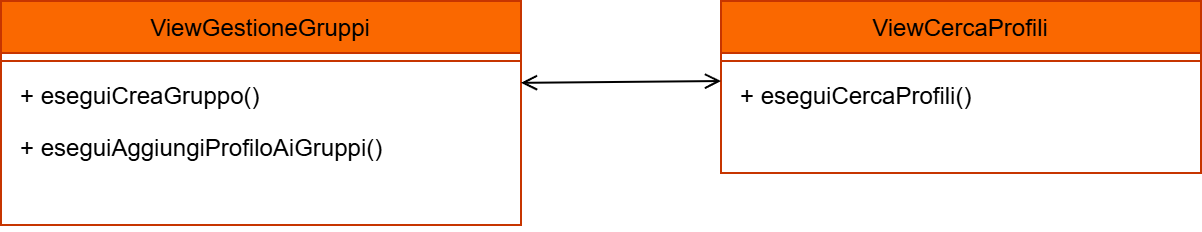
\includegraphics[width=\textwidth]{ProgettoViewGruppi.png}
        \caption{Diagramma di dettaglio delle interfacce di gestione dei gruppi}
    \end{center}
\end{figure}

L'interfaccia della gestione dei gruppi ha il compito di presentare tutti i gruppi 
associati al profilo attualmente in uso,
fornendo l'accesso alle azioni relative. 
Li elenca quindi in maniera chiara, definendo la differenza tra gruppi di due o più persone.
Per ognuno mostra un bottone dal quale, se selezionato, compariranno le azioni attuabili sul gruppo 
(ad esempio, di aggiungere un profilo).\\
\\
\begin{figure}[htbp]
    \centering
    \begin{subfigure}{0.49\textwidth}
        \centering
        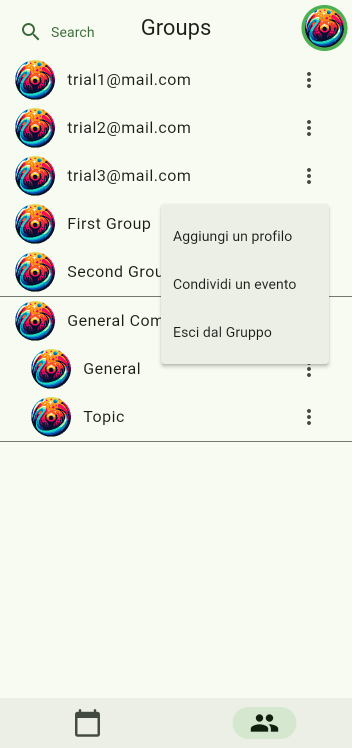
\includegraphics[height=11.5cm, keepaspectratio]{gruppi.png}
        \caption{Elenco dei gruppi}
    \end{subfigure}
    \hfill
    \begin{subfigure}{0.49\textwidth}
        \centering
        
\includegraphics[height=11.5cm, keepaspectratio]{cerca.png}
        \caption{Ricerca dei profili}
    \end{subfigure}
    \caption{Schermate dei gruppi}
\end{figure}

Correlata alla gestione dei profili c'è la loro ricerca, 
che consente il ritrovamento e la successiva aggiunta dei profili tra i propri gruppi.
La schermata risulta minimale, consentendo all'utente di concentrarsi sulle sole informazioni e funzionalità essenziali.\\
\\



\clearpage

La visualizzazione degli eventi prevede due componenti principali.\\
\\
Il primo consiste in una panoramica generale, affiancando gli eventi tra loro a livello settimanale,
per fornire all'utente un quadro complessivo degli impegni. 
Tale vista è ripetuta sia per gli eventi proposti che per quelli confermati, 
con la possibilità di navigare tra le due schermate.\\
\\
Il secondo entra nel particolare dell'evento, 
mostrando i dettagli relativi e fornendo la possibilità di modificarli. 
Concentra inoltre le principali funzionalità dell'applicazione, 
quali la conferma della partecipazione all'evento, la condivisione con i gruppi e il caricamento delle immagini.\\
\\

\begin{figure}[h!]
    \begin{center}
        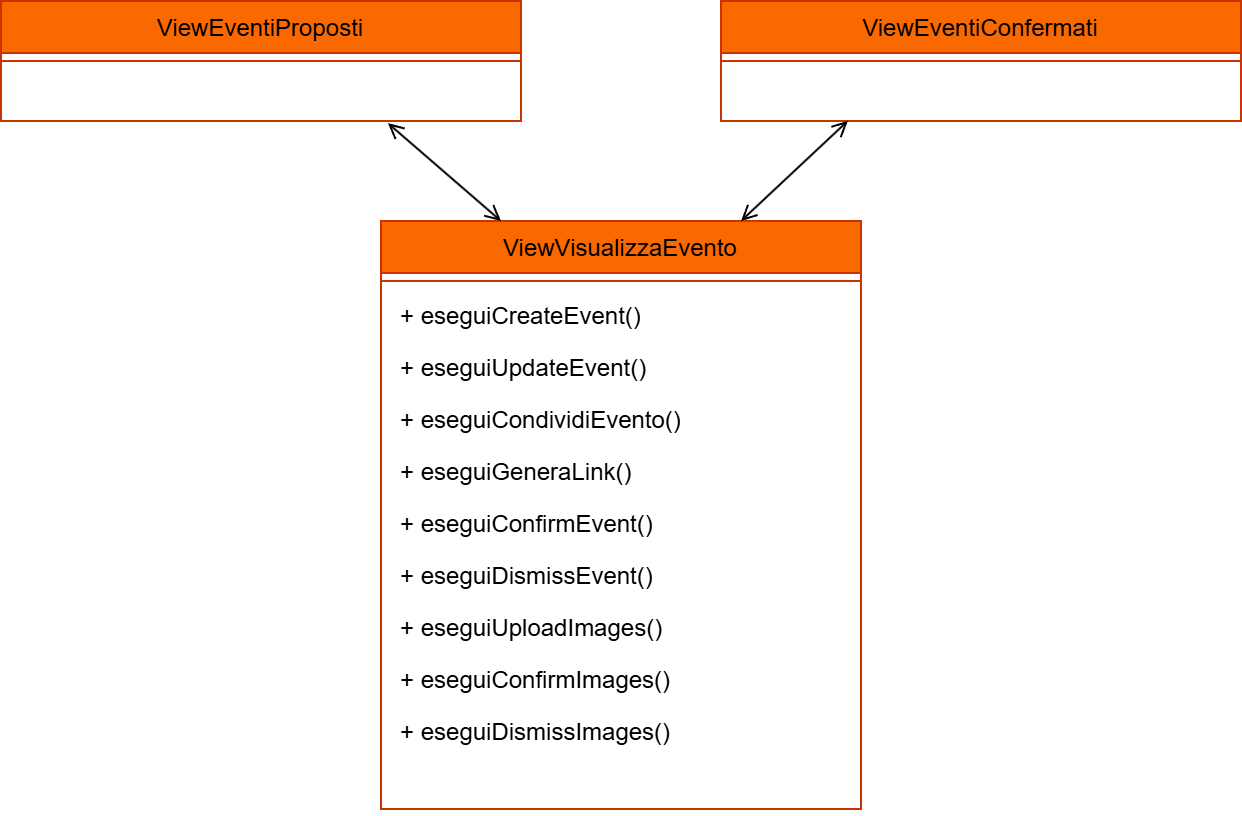
\includegraphics[width=\textwidth]{ProgettoViewEventi.png}
        \caption{Diagramma di dettaglio delle interfacce di visualizzazione eventi}
    \end{center}
\end{figure}
\clearpage

Queste due funzionalità sono al centro del servizio del sistema, 
ed è quindi essenziale che l'interfaccia proposta sia veloce ma sopratutto intuitiva.
Fondamentale in questo riguardo è l'importanza data dai colori, attraverso i quali
ogni elemento risalta in base alla sua importanza, e fornisce il suo contesto e le sue proprietà 
grazie al puro impatto visivo.\\
\\



\begin{figure}[htbp]
    \centering
    \begin{subfigure}{0.49\textwidth}
        \centering
        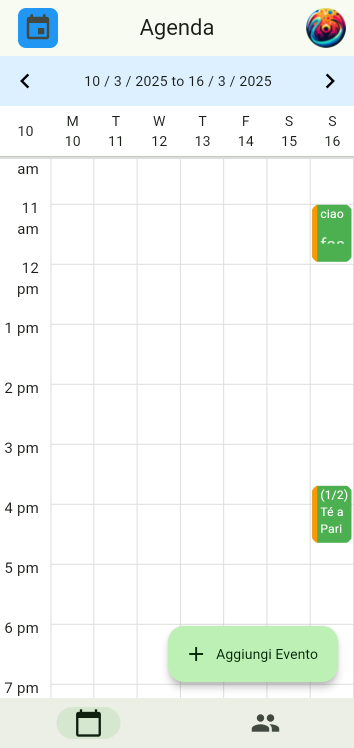
\includegraphics[height=11.5cm, keepaspectratio]{agenda.png}
        \caption{Visualizzazione generale degli eventi}
    \end{subfigure}
    \hfill
    \begin{subfigure}{0.49\textwidth}
        \centering
        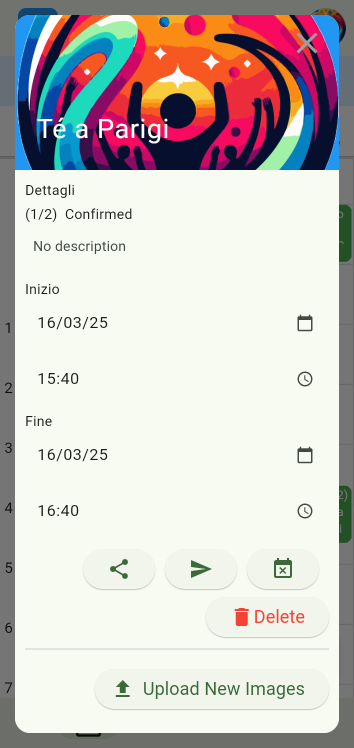
\includegraphics[height=11.5cm, keepaspectratio]{evento.png}
        \caption{Dettaglio di un evento}
    \end{subfigure}
    \caption{Schermate degli eventi}
\end{figure}

\clearpage


\subsection{L'implementazione della logica applicativa}

Ogni interazione con l'utente scatena una qualche forma di elaborazione di dati. 
La visualizzazione di qualunque componente comporta il ritrovamento delle informazioni, 
la loro modifica necessita di essere salvata e la loro condivisione esige la propagazione degli aggiornamenti.
Inoltre, alcuni casi d'uso richiedono azioni da svolgere in autonomia.
L'implementazione della logica necessaria, 
per rispondere efficacemente ai requisiti di velocità ed efficienza,
avviene tramite la creazione di diversi componenti.\\
\\
La suddivisione del programma individua e raggruppa le funzionalità in base al loro contesto, 
affidando a ogni componente meno responsabilità possibili.
Questo permette di concentrare le logiche condivise, 
evitando duplicazioni e definendo chiaramente il ruolo di ogni metodo.
La semplicità del codice così raggiunta semplifica il futuro sviluppo e la sua manutenzione.\\
\\
La principale suddivisione dei componenti avviene in base agli elementi del dominio.
Per ogni principale entità, infatti, viene creato un servizio che ne racchiude
le richieste di ritrovamento, modifica e salvataggio correlate.
Collegando i servizi al dominio si concentrano anche le eventuali dipendenze da altri servizi, 
riducendole alle sole inerenti all'elemento specifico, 
mantenendo un parallelismo logico anche a livello di relazione.\\
\\
La maggior parte delle richieste che riguardano gli elementi del dominio prevede 
la comunicazione con il server esterno. 
La ricezione e l'aggiornamento dei dati, così come la permanenza delle modifiche, avviene infatti attraverso 
l'interazione con la persistenza principale, a cui si può accedere tramite il server.
Vista la complessità specifica nella creazione delle trasmissioni e 
la loro secondaria importanza a livello logico, 
vengono realizzati dei componenti dedicati, chiamati API.
I componenti API permettono quindi l'astrazione delle trasmissioni con il server, 
semplificando il codice e 
separando la logica applicativa dalle complessità richieste dalla tecnologia dei protocolli usata.

\clearpage 

\begin{figure}[h!]
    \begin{center}
        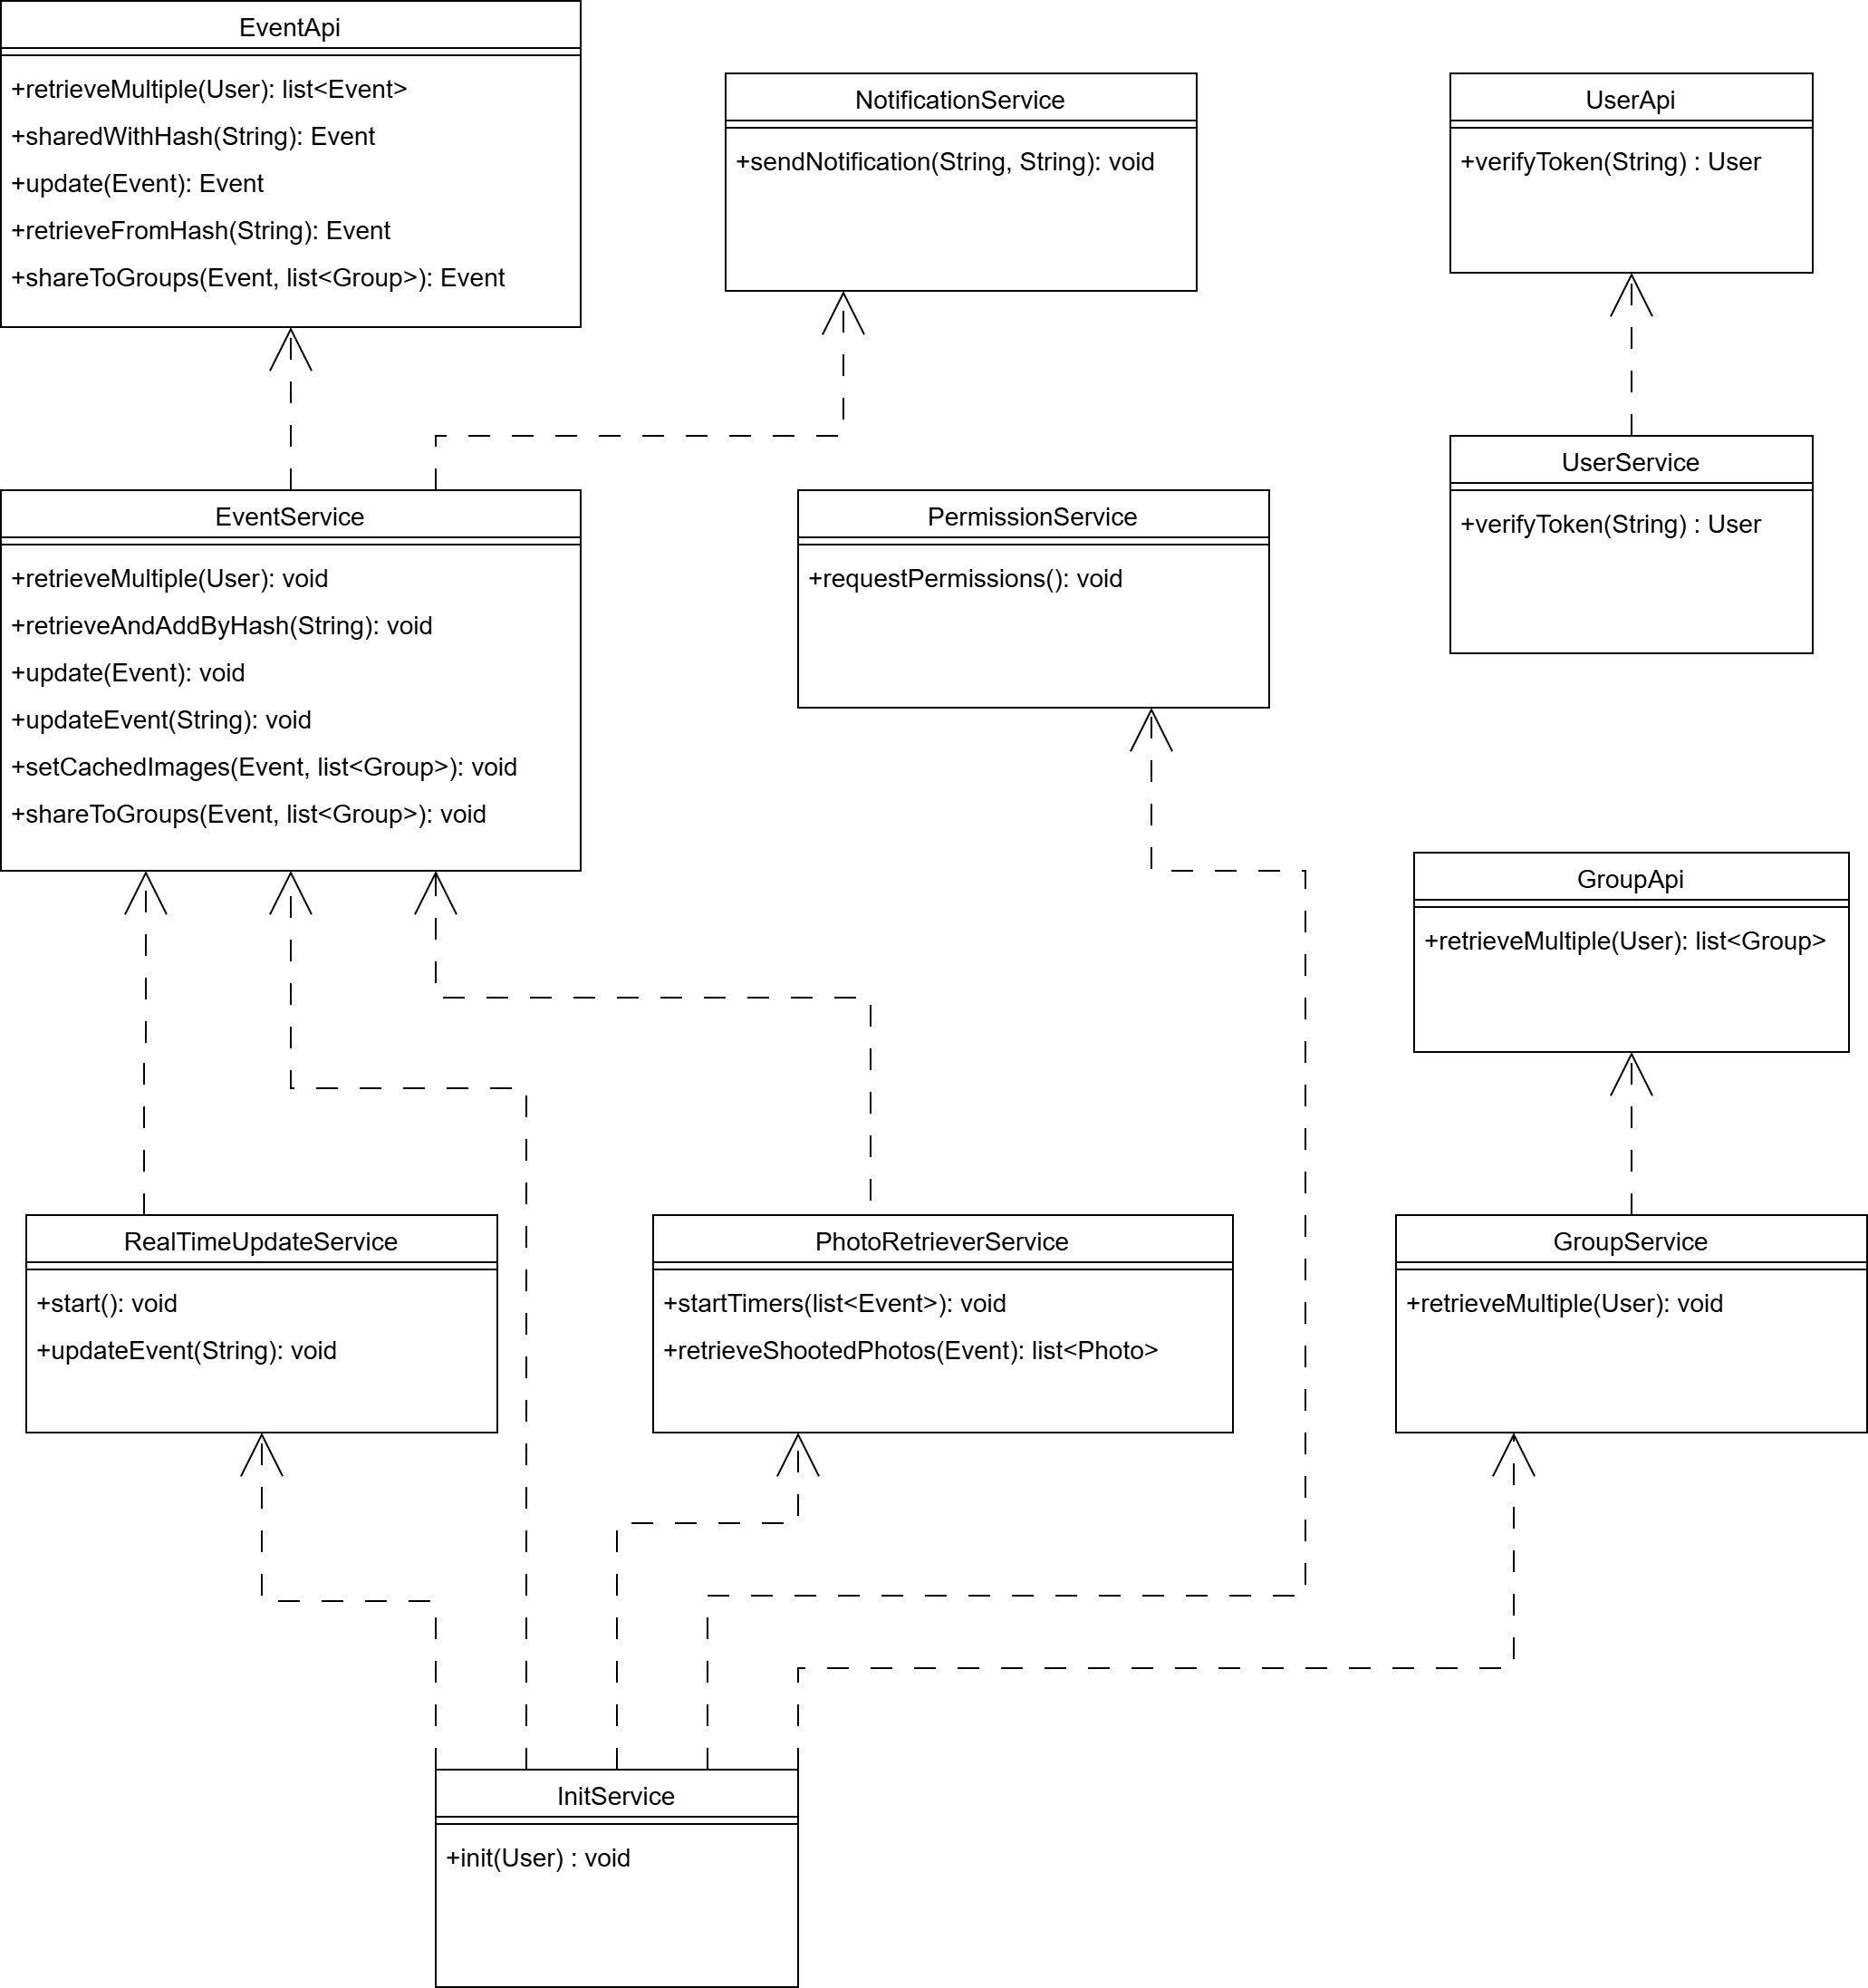
\includegraphics[width=\textwidth]{FrontServiceClassDiagram.png}
        \caption{Modello delle classi del client}
    \end{center}
\end{figure}

Non tutte le funzionalità sono però correlate direttamente al dominio.
Per questo motivo si creano servizi ausiliari dedicati, 
anch'essi separatati in base al ruolo che ricoprono.
\clearpage
Un servizio è stato dedicato all'acquisizione e 
al salvataggio dei permessi necessari per operare, 
quali l'invio delle notifiche e l'accesso alla galleria. 
Mette a disposizione degli altri processi, quindi, la conferma dell'accesso ai permessi richiesti o, 
in caso non lo si possegga, gestirà il suo ottenimento.\\ 
\\
L'invio delle notifiche e la ricezione degli aggiornamenti, 
per quanto concettualmente simili e strettamente correlati,
sono stati implementati in due componenti differenti. 
Le notifiche possono essere infatti richieste anche da altri metodi, 
e a ogni aggiornamento potrebbe non corrispondere una notifica.
La ricezione delle modifiche in tempo reale avviene usando il pattern observer, 
nel quale il servizio si connette a un canale e rimane in attesa di eventuali messaggi.

\begin{figure}[h!]
    \begin{center}
        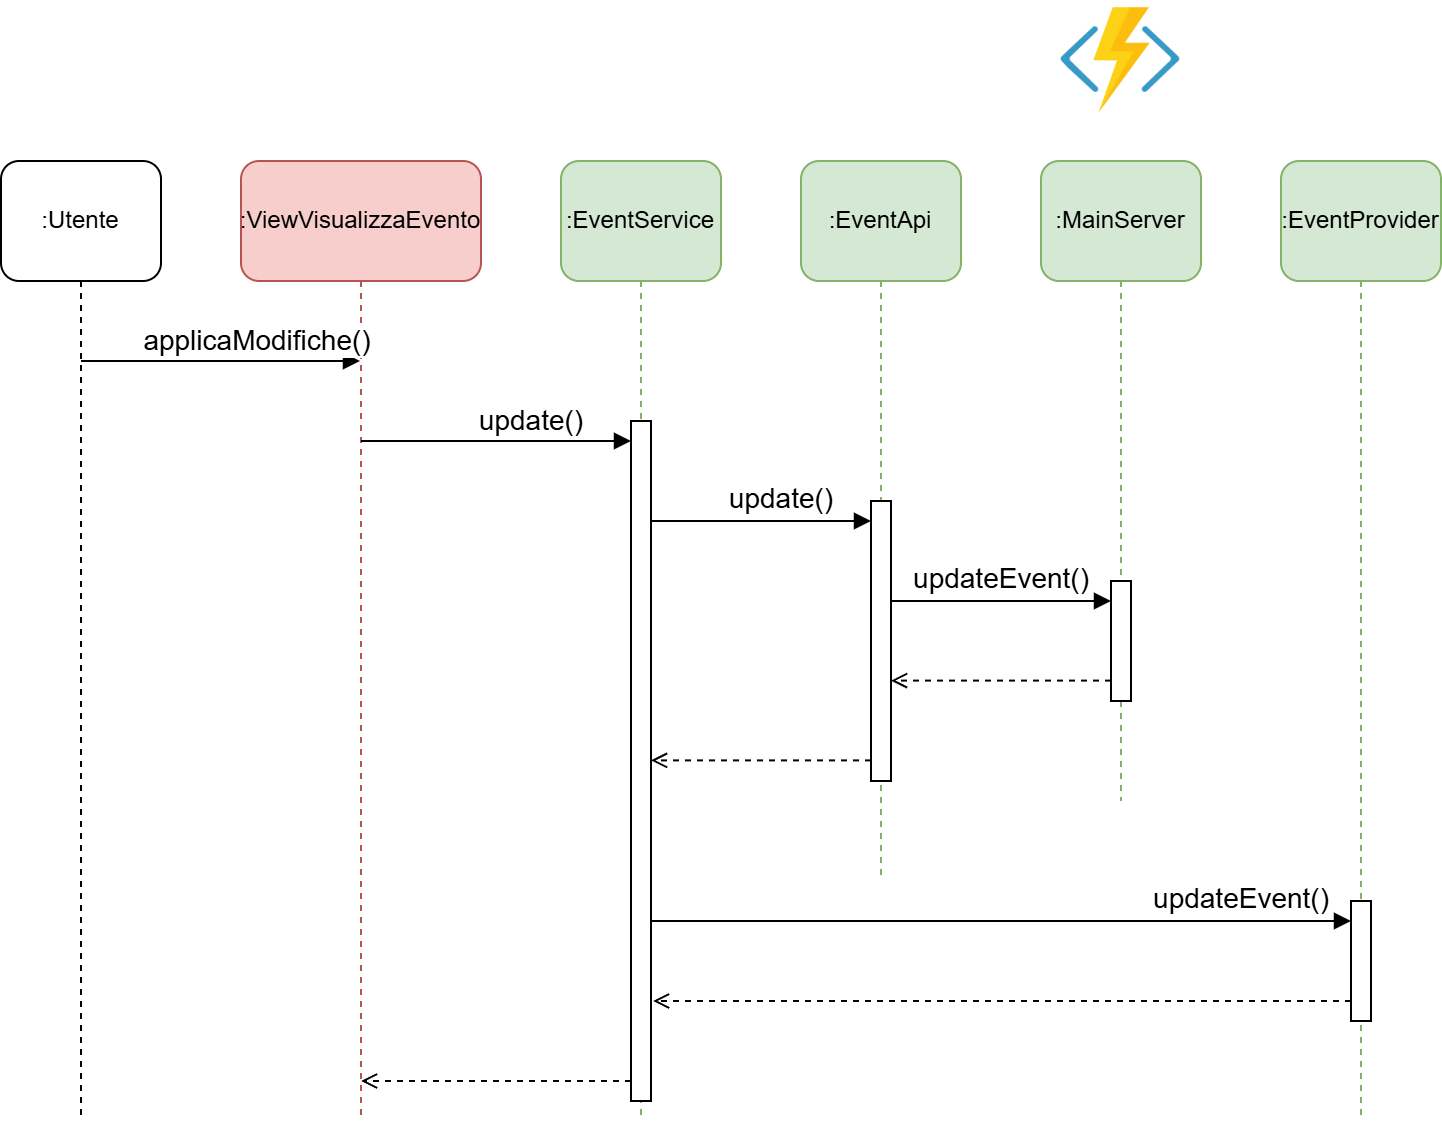
\includegraphics[width=\textwidth]{IIModificaEvento1.png}
        \caption{Diagramma di sequenza della modifica di un evento}
    \end{center}
\end{figure}

\clearpage

Il salvataggio in memoria locale dei dati risulta fondamentale per la reattività dell'applicazione,
in quanto permette di ridurre le richieste di dati e velocizza il loro recupero.
La memoria locale viene implementata grazie a classi Provider, create in relazione agli elementi del dominio.
Un'altra funzionalità centrale dell'applicazione è il recupero automatico 
delle foto scattate durante l'evento. 
Questo richiede la pianificazione di azioni automatiche nel tempo,
così come la scansione della galleria per trovare le immagini interessate.
Sia la gestione locale della memoria che il recupero delle immagini vedono uno o più componenti dedicati.
La loro realizzazione viene trattata nei capitoli seguenti.\\
\\
Durante l'implementazione della logica applicativa si sono dovuti affrontare altri problemi quali, degni di nota, 
la gestione della condivisione di un evento tramite link e l'inizializzazione dell'applicazione.\\

\begin{figure}[h!]
    \begin{center}
        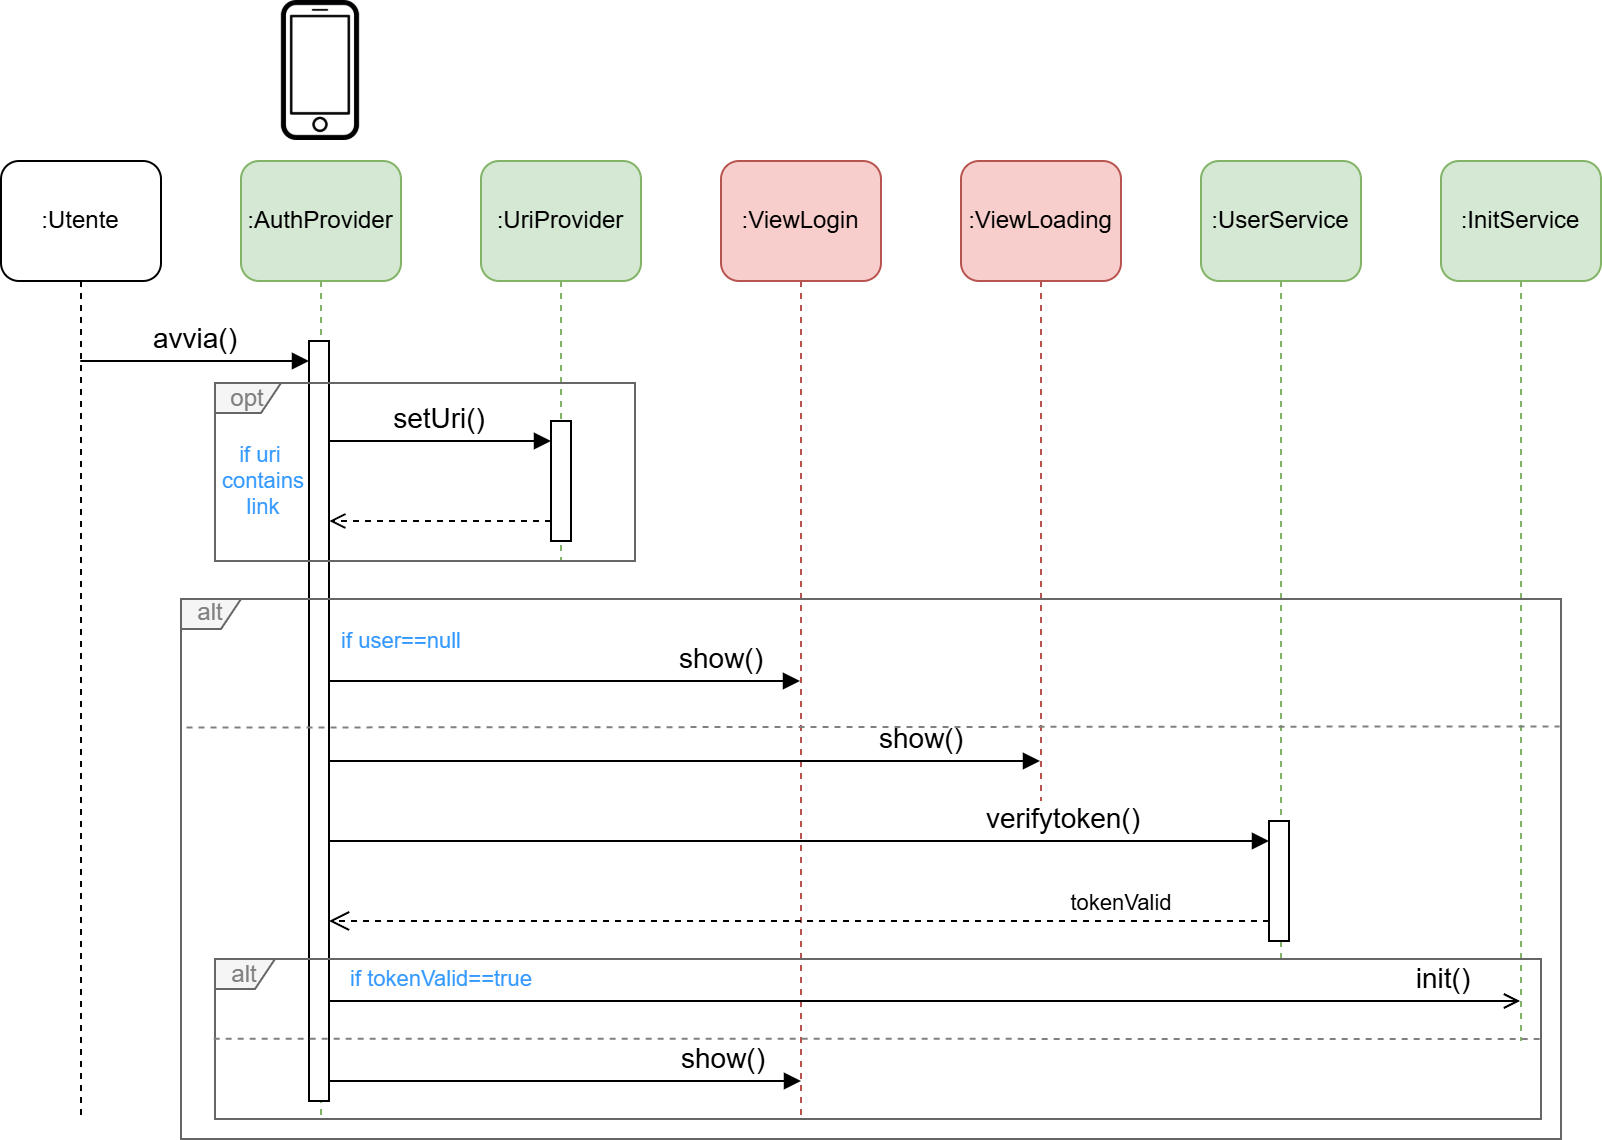
\includegraphics[width=\textwidth]{Avvio.png}
        \caption{Diagramma di sequenza dell'avvio dell'applicazione}
    \end{center}
\end{figure}

La condivisione di un evento tramite link consiste in due passaggi principali: 
la creazione del link stesso e il successivo ritrovamento dell'evento associato.
La generazione del link avviene tramite l'unione del dominio del server con il codice identificativo dell'evento.
\clearpage
All'apertura dell'applicazione tramite link viene estratto il codice identificativo dell'evento 
per la successiva richiesta dei dati al server.
Se l'utente non si è ancora autenticato, però, il router dell'applicazione lo reindirizza alla schermata di login, 
cambiando il link e perdendo l'informazione allegata.
Per evitare questo problema, nel momento in cui l'utente accede all'applicazione tramite un link,
le sue informazioni vengono salvate in memoria locale.
Al termine del login, se sono presenti dati salvati, l'utente verrà indirizzato alla schermata degli eventi proposti, 
che recupererà i dati relativi all'evento, per poi mostrarli a video.

\begin{figure}[h!]
    \begin{center}
        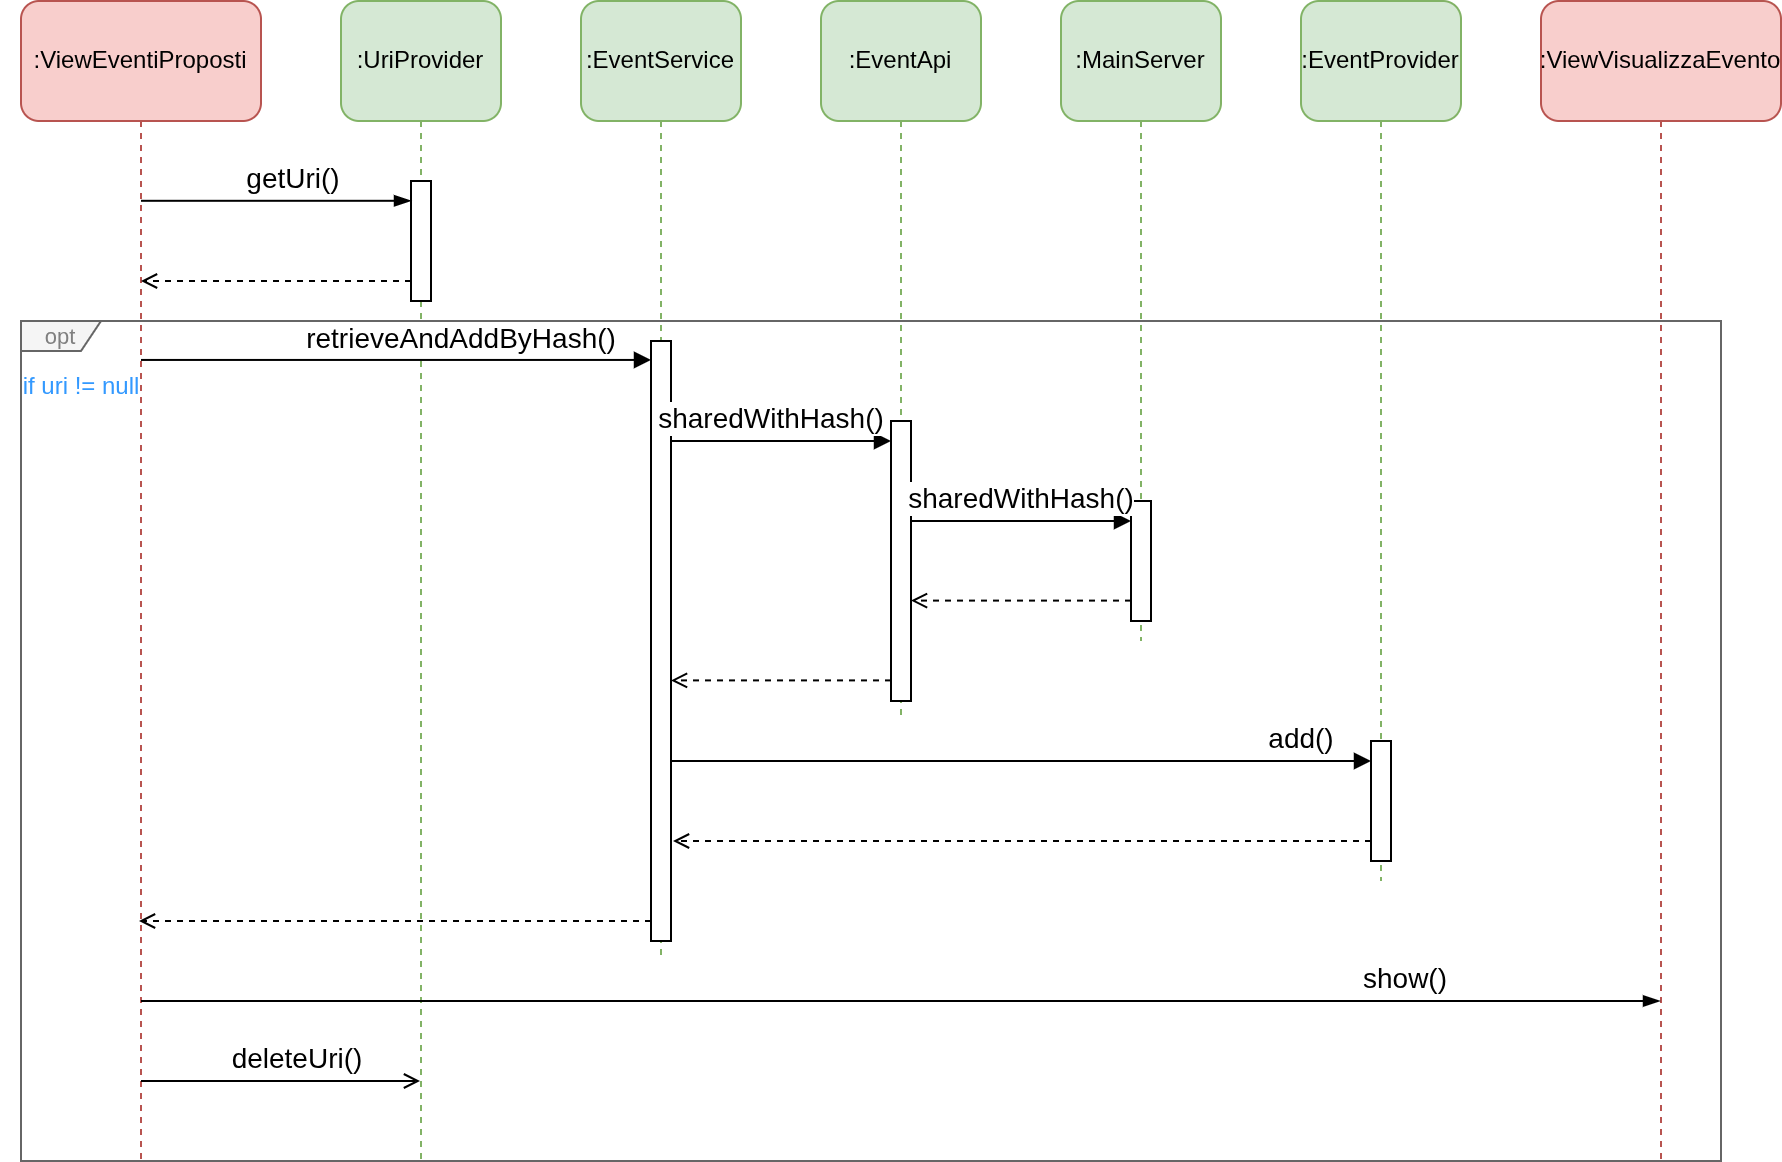
\includegraphics[width=\textwidth]{IIVisualizzaEventiProposti.png}
        \caption{Diagramma di sequenza della visualizzazione degli eventi proposti}
    \end{center}
\end{figure}

\clearpage

La fase di inizializzazione avviene a seguito di un login andato a buon fine.
Parallelamente alla visualizzazione della schermata iniziale si recuperano i dati 
relativi ai profili associati all'utente e vengono fatti partire i servizi autonomi. 
In particolare, vengono controllati i permessi necessari per i quali, se non ancora concessi, 
verrà richiesto l'ottenimento. 
Viene inoltre avviato il servizio di ricezione degli aggiornamenti, che si connette al canale relativo all'utente.
Per ogni profilo vengono, sempre in maniera parallela, recuperati i gruppi e gli eventi associati.
Al termine della ricezione degli eventi, indipendentemente dalle altre richieste, 
per ogni evento successivo al momento attuale viene avviato un timer, che scatena, 
al momento giusto, il recupero delle immagini.
Se l'applicazione è stata aperta tramite link di condivisione, 
la schermata a cui si verrà reindirizzati sarà quella degli eventi proposti, altrimenti quella degli eventi confermati.\\
\\

\begin{figure}[h!]
    \begin{center}
        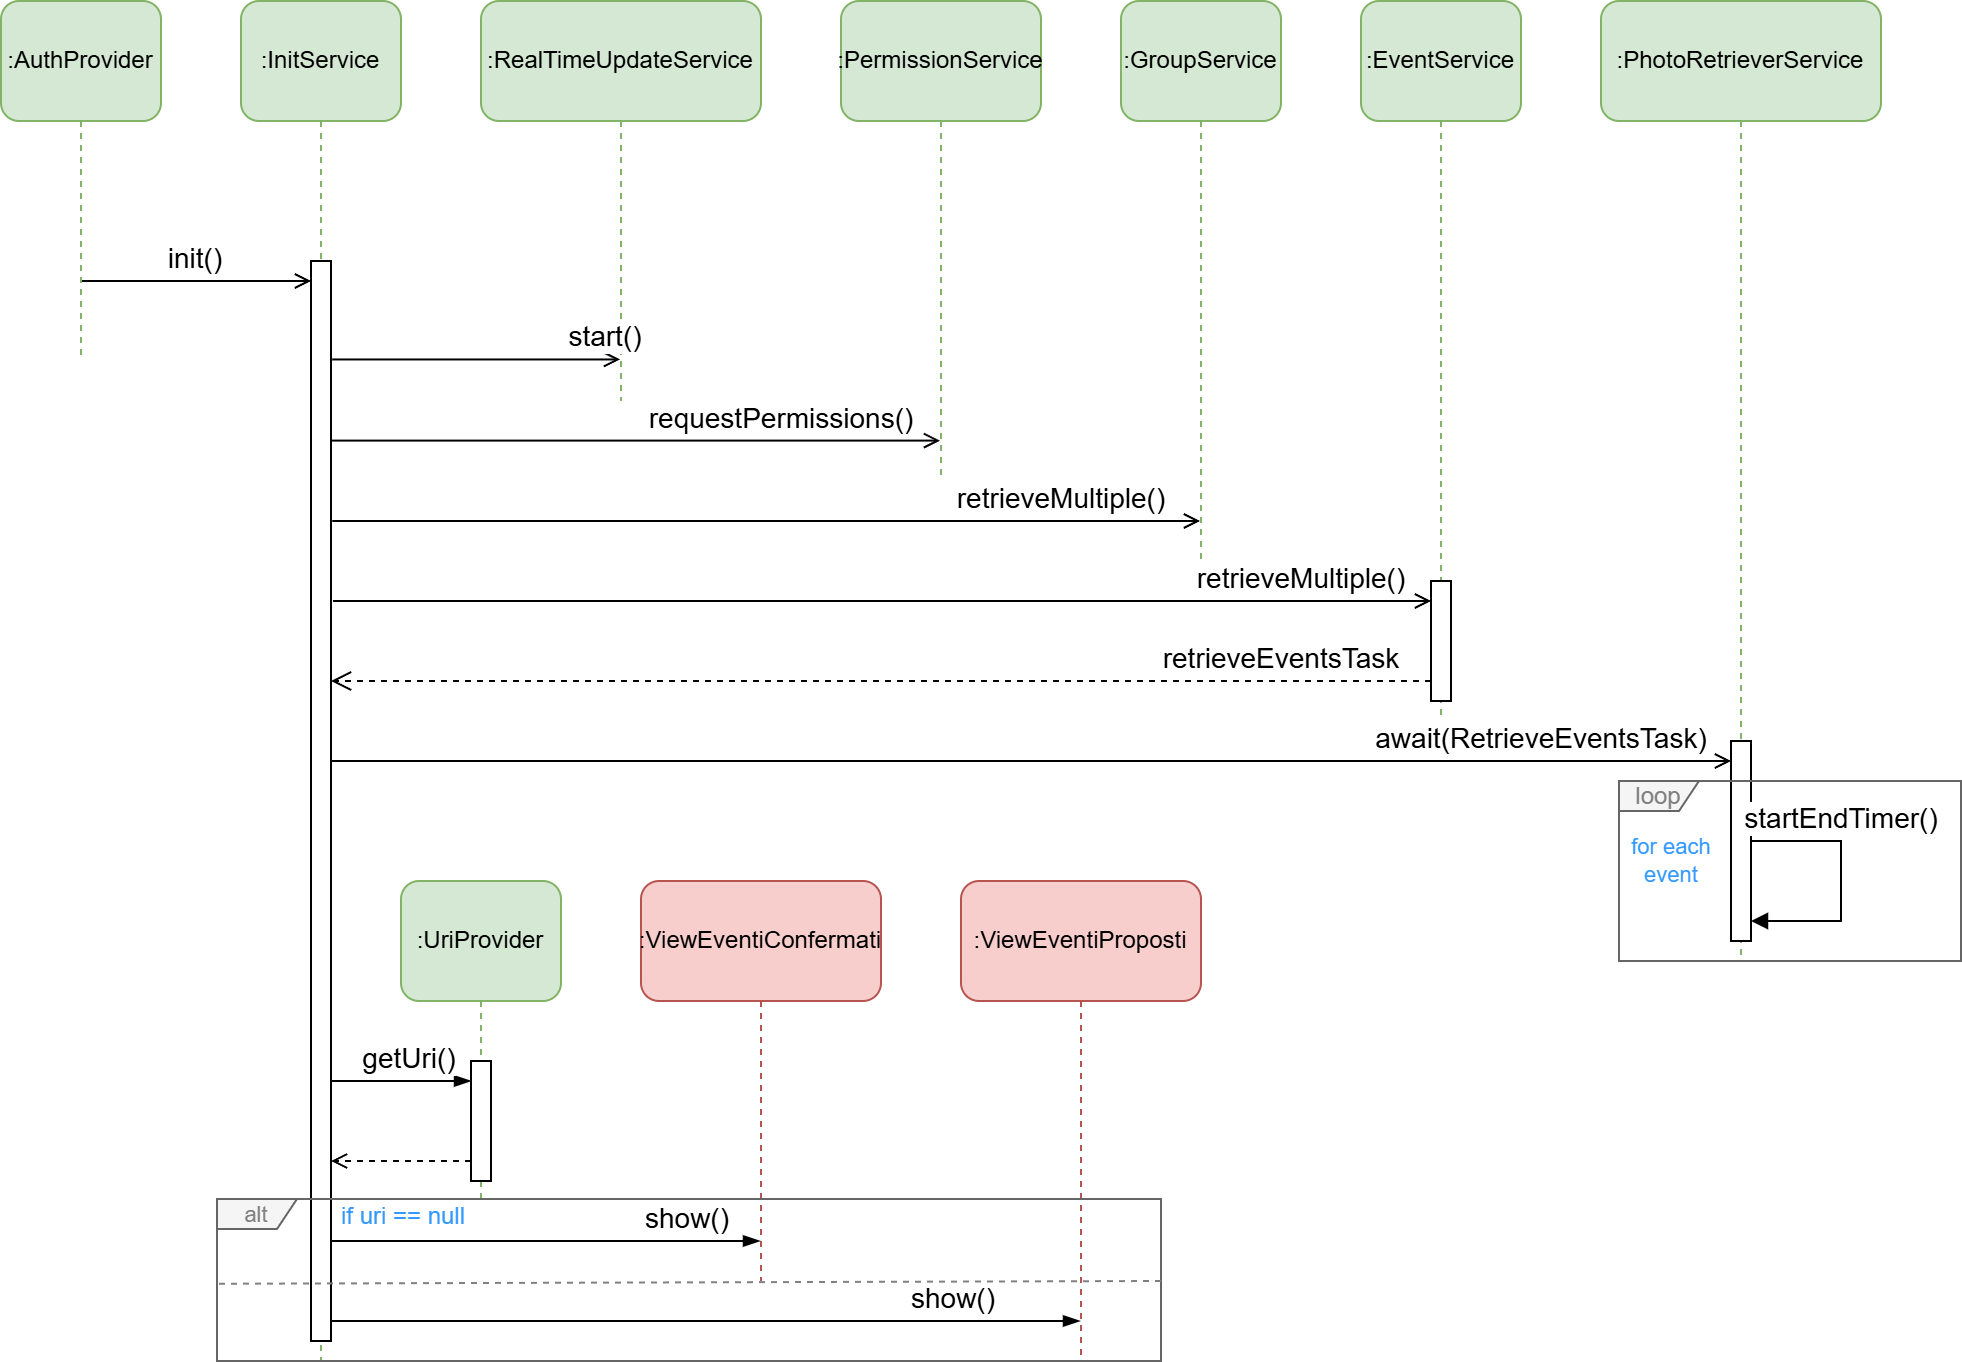
\includegraphics[width=\textwidth]{Init.png}
        \caption{Diagramma di sequenza della fase di inizializzazione }
    \end{center}
\end{figure}


\clearpage

\subsection{La distribuzione del codice verso i dispositivi utente}

Per quanto Flutter consenta di uniformare l'esperienza utente su dispositivi diversi e 
semplifichi la compilazione per le varie piattaforme,
alcune configurazioni rimangono comunque dipendenti dalla tecnologia su cui l'applicazione viene eseguita.
Di conseguenza, ciascun eseguibile richiede una manutenzione aggiuntiva, 
inclusi gli aggiornamenti delle dipendenze specifiche,
sia a livello di deployment che di gestione delle versioni.
Per questi motivi, nella fase iniziale dello sviluppo,
nell'ottica di coprire il più ampio mercato possibile con il minor numero di piattaforme,
si è deciso di sviluppare una versione fruibile via web e una per dispositivi Android, 
con l'obiettivo di estendere il servizio alle altre tecnologie in un secondo momento.\\
\\
La grafica è stata sviluppata in maniera statica, 
ovvero non dipende direttamente da nessuna informazione specifica dell'utente.
L’interfaccia sviluppata infatti non prevede la creazione dinamica di contenuti:
gli elementi visuali che vengono restituiti rimangono invariati indipendentemente dall'utente che ne effettua la richiesta.
I dati visualizzati che interessano l'utente corrente (eventi confermati o proposti, gruppi, profili e via dicendo)
sono recuperati dalla memoria locale del dispositivo o tramite un server terzo.
Questa scelta consente di rendere l'interfaccia grafica completamente indipendente dall'identità o dal ruolo dell'utente,
consentendo una separazione netta delle responsabilità dei componenti.\\
\\
Da un punto di vista della distribuzione,
le due tecnologie per cui l'interfaccia è stata realizzata funzionano in modalità completamente diversa.
L'interfaccia web prevede l'utilizzo di un browser utente che si connette a un server apposito
per ottenere la grafica da visualizzare.
L'interfaccia Android (come qualunque interfaccia realizzata per essere eseguita direttamente su un dispositivo)
richiede invece la creazione di un applicativo apposito, 
da scaricare e installare sul dispositivo.\\
\\
Per la fruizione del codice web si necessita di un server relativamente semplice,
che, grazie alla staticità del sito, 
restituisca solo gli elementi necessari per la visualizzazione e l'elaborazione locale,
senza bisogno di modificarli.
La creazione di questo tipo di risorsa usando tecnologie in cloud può avvenire in vari modi,
dall'utilizzo di una macchina virtuale apposita a soluzioni che utilizzano container.
Tuttavia, Azure mette a disposizione un servizio apposito per queste precise esigenze,
Azure Static Web App (ASWA).\\
\\
Questa risorsa, oltre a integrarsi direttamente con il resto dell'ambiente Azure,
permettendo quindi (ad esempio) il collegamento con servizi di monitoraggio delle performance,
garantisce disponibilità e scalabilità in ogni momento,
facendosi carico di gestire la capacità computazionale richiesta.
Il consumo delle risorse è infatti calcolato in base alla bandwidth, 
ovvero la quantità di dati che viene fornita dal server.
Il piano gratuito prevede i primi cento giga byte di bandwidth inclusi,
che rende il servizio vantaggioso, oltre che pratico.\\
\\
La distribuzione dell'applicativo Android 
necessita di un modo per scaricare il file di installazione del programma.
In attesa della pubblicazione dell'applicativo sull'App Store di Android, 
che fornirebbe agli utenti la possibilità di trovarlo e installarlo direttamente,
ma che richiede ulteriori passaggi di certificazione e autenticazione,
è stato necessario trovare un'altra soluzione.
Anche in questo caso, 
le opzioni per fornire un file tramite cloud ce ne sono tante,
ma la più semplice ed efficace è attraverso l'utilizzo di Azure Blob Storage.\\
\\
Questo servizio consente l'archiviazione e la distribuzione di file di varie tipologie,
fornendo un link diretto per il loro recupero.
Ha un costo che varia in base all'utilizzo, 
aggirandosi attorno ai due centesimi per giga byte.
Bilanciando la temporaneità del servizio,
la ridotta quantità di download inizialmente previsti e
la complessità che verrebbe introdotta in caso di utilizzo di un altro servizio,
non è stato ritenuto necessario approfondire ulteriormente la ricerca.\\
\\
Nonostante l'esecuzione del codice presenti alcune dipendenze in base al dispositivo,
la distribuzione non ha introdotto nessuna necessità.
Nessuna modifica del codice è stata quindi dovuta alla scelta della tecnologia usata per 
la loro distribuzione.\\
\\

\begin{figure}[h!]
    \begin{center}
        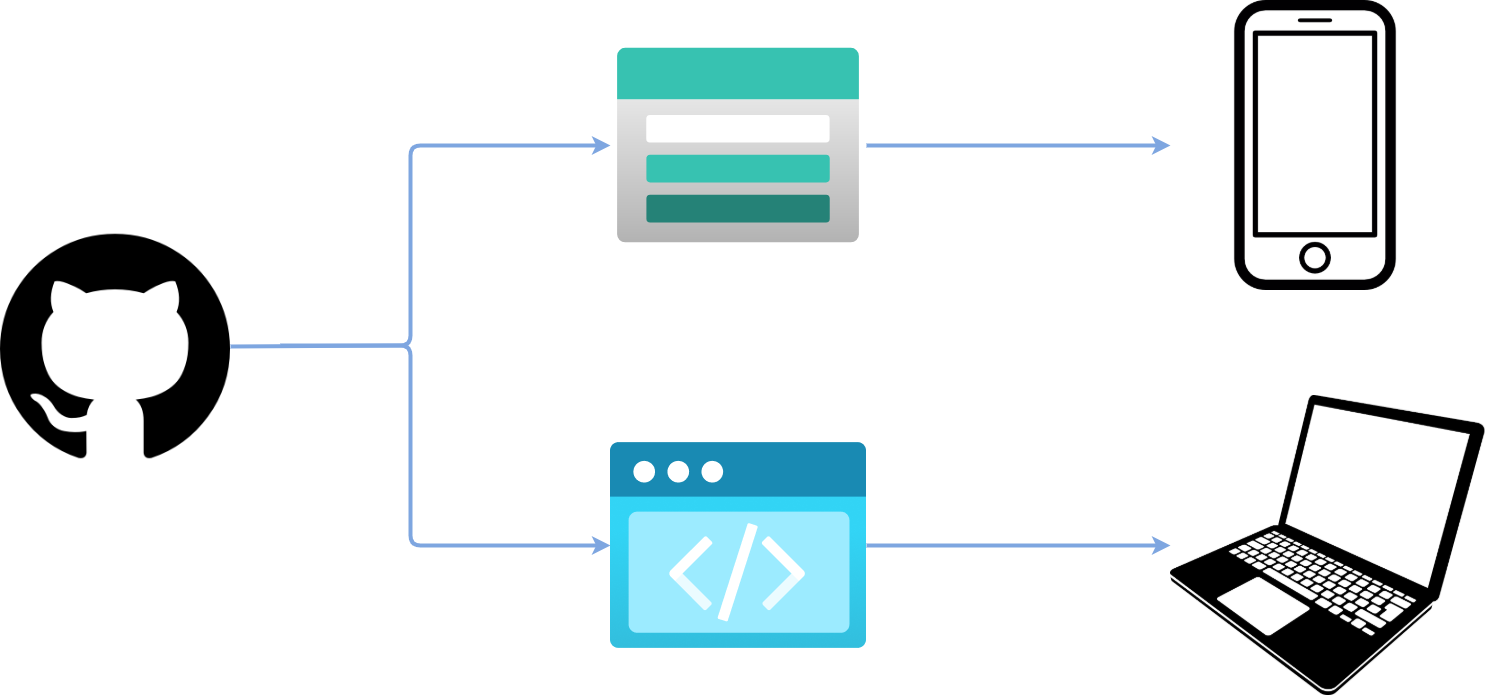
\includegraphics[height=0.28\textheight]{DeployFront.png}
        \caption{Diagramma di aggiornamento e distribuzione del client}
    \end{center}
\end{figure}

Per garantire un processo di aggiornamento efficiente e automatizzato,
sia il codice distribuito sulla web app che l'applicativo ospitato nel container 
vengono gestiti tramite GitHub Actions.
Le Github Actions sono funzionalità offerte da Github, 
che è il sito dove viene salvato il codice.
In particolare, a ogni nuova versione del codice sia la Static Web App che il Blob Storage vengono notificati,
modificando il loro contenuto.
Questo consente di offrire un servizio aggiornato 
riducendo al minimo i tempi richiesti per applicare le modifiche. 
ASWA gestisce in autonomia il collegamento con la repository Github, 
mentre per aggiornare l'applicazione su Android è stato necessario crearne una appositamente.\\
\\
In caso di aggiornamento, 
la fruizione dell'interfaccia tramite browser non necessita di nessuna manutenzione 
in quanto si aggiorna automaticamente a ogni accesso.
Per l'applicativo su dispositivo mobile è invece necessaria una nuova installazione manuale.
Per questa ragione, gli utenti dell'applicazione verranno notificati tempestivamente 
ogni volta che sarà disponibile una nuova versione.
\clearpage
